\section{Calibration by Simulation}


We consider an economy with a continuum of firms indexed by $i$. Each firm $i$ has idiosyncratic productivity $z_{it}$ and chooses labor demand $\ell_{it} \ge 0$. Output is produced with a Cobb-Douglas technology in productivity and labor:
\begin{equation}
  y_{it} = (z_{it})^{1-\eta}\, (\ell_{it})^{\eta},
\end{equation}
where $\eta \in (0,1)$. In a partial equilibrium setting we normalize the wage $W = 1$. The firm's problem is
\begin{equation}
  \max_{\ell_{it} \ge 0} \quad y_{it} - W \ell_{it} = (z_{it})^{1-\eta}\, (\ell_{it})^{\eta} - \ell_{it}.
\end{equation}
The first-order condition $\eta\, (z_{it})^{1-\eta}\, (\ell_{it})^{\eta-1} = 1$ yields optimal labor
\begin{equation}
  \ell_{it} = \eta^{1/(1-\eta)}\, z_{it},
\end{equation}
and therefore output
\begin{equation}
  y_{it} = (z_{it})^{1-\eta}\, \bigl(\eta^{1/(1-\eta)}\, z_{it}\bigr)^{\eta}
  = \eta^{\eta/(1-\eta)}\, z_{it}.
\end{equation}
Hence $\log y_{it} = \log z_{it} + \text{const}$: (log) output and (log) productivity coincide up to a constant. We observe a panel of log productivity (or log output) and seek to calibrate the parameters of the stochastic process that governs $\log z_{it}$ by matching selected moments.

\subsection{Stochastic process for log productivity}

We drop the firm index $i$ when describing the law of motion. Let $y_t \equiv \log z_{it}$ denote log productivity (or log output) and $x_t \equiv \log \hat z_{it}$ the persistent component. The process is
\begin{align*}
  y_t &= x_t + \varepsilon_t, \qquad \varepsilon_t \stackrel{\text{iid}}{\sim} \mathcal{N}(0,\sigma_\varepsilon^2), \\
  x_t &= \rho x_{t-1} + u_t, \qquad u_t \stackrel{\text{iid}}{\sim} \mathcal{N}(0,\sigma_u^2), \qquad |\rho| < 1, \\
  u_t &\perp \varepsilon_s \quad \forall t,s.
\end{align*}
So log productivity is the sum of a persistent AR(1) component $x_t$ and an iid transitory shock $\varepsilon_t$.

\subsection{Analytical moments}

\subsubsection{Variance and standard deviation of $\log y_t$}

The persistent component has stationary variance $\Var(x_t) = \sigma_u^2/(1-\rho^2)$. Hence
\begin{align*}
  \Var(y_t) &= \Var(x_t) + \Var(\varepsilon_t)
  = \frac{\sigma_u^2}{1-\rho^2} + \sigma_\varepsilon^2, \\
  \operatorname{sd}(y_t) &= \sqrt{\frac{\sigma_u^2}{1-\rho^2} + \sigma_\varepsilon^2}.
\end{align*}

\subsubsection{Variance and standard deviation of $\Delta y_t \equiv y_t - y_{t-1}$}

Using $\Var(\Delta y_t) = 2\Var(y_t) - 2\Cov(y_t,y_{t-1})$ and $\Cov(y_t,y_{t-1}) = \Cov(x_t,x_{t-1}) = \rho \Var(x_t) = \rho \sigma_u^2/(1-\rho^2)$,
\begin{align*}
  \Var(\Delta y_t)
  &= 2\left(\frac{\sigma_u^2}{1-\rho^2}+\sigma_\varepsilon^2\right)
  - 2\,\rho\,\frac{\sigma_u^2}{1-\rho^2}
  = 2\left(\frac{\sigma_u^2}{1+\rho}+\sigma_\varepsilon^2\right), \\
  \operatorname{sd}(\Delta y_t) &= \sqrt{2\left(\frac{\sigma_u^2}{1+\rho}+\sigma_\varepsilon^2\right)}.
\end{align*}

\subsubsection{Autocorrelations of $\log y_t$}

For $k \ge 1$,
\begin{align*}
  \Cov(y_t,y_{t-k})
  &= \Cov(x_t,x_{t-k})
  = \rho^k \Var(x_t)
  = \rho^k \,\frac{\sigma_u^2}{1-\rho^2}, \\
  \Corr(y_t,y_{t-k})
  &= \frac{\Cov(y_t,y_{t-k})}{\Var(y_t)}
  = \rho^k \cdot \frac{\frac{\sigma_u^2}{1-\rho^2}}{\frac{\sigma_u^2}{1-\rho^2}+\sigma_\varepsilon^2}.
\end{align*}
We target the autocorrelations at lags $k=1$, $3$, and $5$:
\begin{align*}
  \Corr(y_t,y_{t-1}) &= \rho \cdot \frac{\frac{\sigma_u^2}{1-\rho^2}}{\frac{\sigma_u^2}{1-\rho^2}+\sigma_\varepsilon^2}, \\
  \Corr(y_t,y_{t-3}) &= \rho^3 \cdot \frac{\frac{\sigma_u^2}{1-\rho^2}}{\frac{\sigma_u^2}{1-\rho^2}+\sigma_\varepsilon^2}, \\
  \Corr(y_t,y_{t-5}) &= \rho^5 \cdot \frac{\frac{\sigma_u^2}{1-\rho^2}}{\frac{\sigma_u^2}{1-\rho^2}+\sigma_\varepsilon^2}.
\end{align*}

\subsection{Simulation and target moments}

We simulate a panel of $N = 100{,}000$ firms over $T = 10$ periods. For each firm we draw the initial persistent component from the ergodic distribution $\mathcal{N}(0,\sigma_u^2/(1-\rho^2))$, then evolve $x_t$ and add iid $\varepsilon_t$ to obtain $y_t = x_t + \varepsilon_t$. From the simulated panel we compute:
\begin{itemize}[leftmargin=*]
  \item standard deviation of $\log y_t$,
  \item standard deviation of the one-year change $\Delta y_t = y_t - y_{t-1}$,
  \item autocorrelations of $y_t$ at lags 1, 3, and 5.
\end{itemize}
We match these to the following target moments (from the data): $\operatorname{sd}(y) = 1.31$, $\operatorname{sd}(\Delta y) = 0.59$, $\Corr(y_t,y_{t-1}) = 0.90$, $\Corr(y_t,y_{t-3}) = 0.87$, $\Corr(y_t,y_{t-5}) = 0.85$.

\Cref{fig:problem3-dlogz} shows the distribution of log-productivity changes at horizons 1, 3, and 5 years from the simulated panel (using initial parameter guesses). Under this two-component process, the change $\Delta_k y_t = y_t - y_{t-k}$ is the sum of two independent normal random variables and is therefore normal; the empirical densities align with this.

\begin{figure}[H]
  \centering
  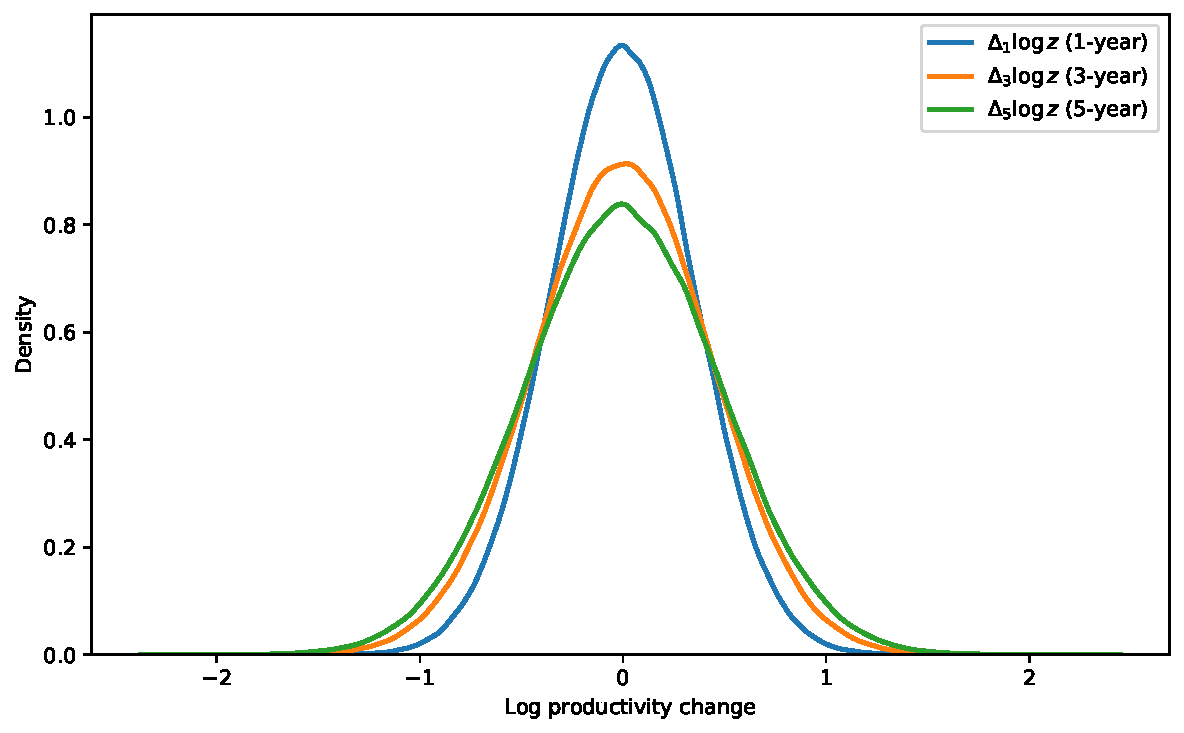
\includegraphics[width=0.75\textwidth]{figures/problem3_dlogz}
  \caption{Distribution of log-productivity changes: density of $\Delta_1 \log z$, $\Delta_3 \log z$, and $\Delta_5 \log z$ from the simulated panel (KDE).}
  \label{fig:problem3-dlogz}
\end{figure}

\subsection{Estimation: Nelder-Mead}

We estimate $\theta = (\rho,\sigma_u,\sigma_\varepsilon)$ by minimizing the sum of squared errors between the five model moments and the five target moments (SSE). We use the Nelder-Mead simplex algorithm (no derivatives), with simple bounds: $\rho \in [0.70, 0.99]$, $\sigma_u,\sigma_\varepsilon \in [0.01, 0.50]$. At each iteration we simulate the panel once (fixed seed for reproducibility) and compute the moments; the objective is the squared Euclidean norm of the moment residual vector.

\Cref{fig:problem3-nelder} plots the SSE at each Nelder-Mead iteration. The algorithm converges to a low SSE, and the resulting parameter vector reproduces the target moments closely (e.g.\ $\hat\rho \approx 0.986$, $\hat\sigma_u \approx 0.21$, $\hat\sigma_\varepsilon \approx 0.39$).

\begin{figure}[H]
  \centering
  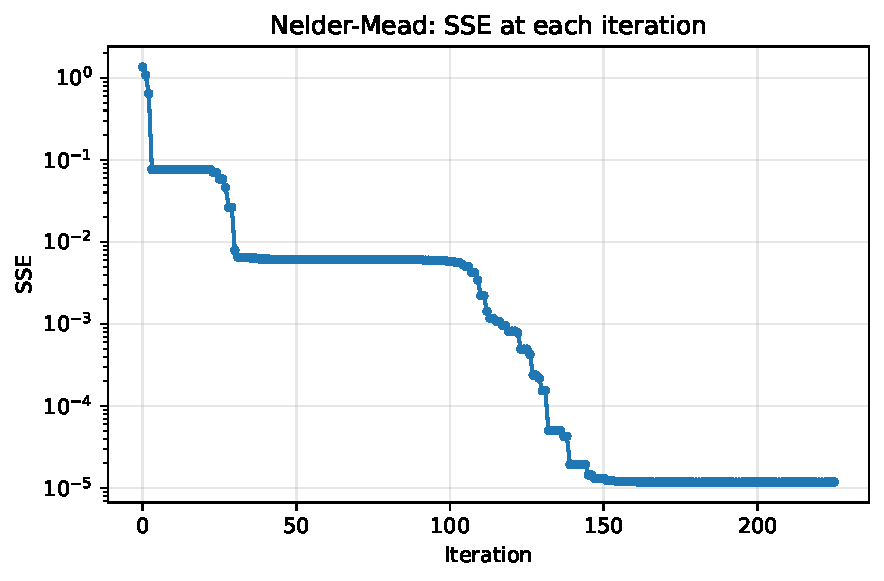
\includegraphics[width=0.65\textwidth]{figures/problem3_nelder_sse}
  \caption{Nelder-Mead: SSE (sum of squared moment errors) at each iteration.}
  \label{fig:problem3-nelder}
\end{figure}

\subsection{Implementation notes}

\begin{itemize}[leftmargin=*]
  \item \textbf{Simulation:} Initial $x_0$ is drawn from $\mathcal{N}(0,\sigma_u^2/(1-\rho^2))$; then $x_t = \rho x_{t-1} + u_t$ and $y_t = x_t + \varepsilon_t$ for $t=1,\ldots,T-1$.
  \item \textbf{Moments:} Standard deviations and correlations are computed from the flattened panel (all firms and time periods used for each moment).
  \item \textbf{Nelder-Mead:} We use \texttt{hetmacro.optimize.nelder\_mead} with \texttt{return\_info=True} to record the objective value at each iteration for the convergence plot.
\end{itemize}

\subsection{Extension: Jump-diffusion (fat tails)}

To capture fat tails and leptokurtic distributions in the data, we extend the persistent component to a \emph{jump-diffusion}. Idiosyncratic log productivity is $\tilde{y}_{it} = x_{it} + \varepsilon_{it}$ with $\varepsilon_{it} \sim \mathcal{N}(0,\sigma_\varepsilon^2)$. The persistent state follows
\begin{align*}
  x_{it} &= \rho x_{i,t-1} + \eta_{it} + J_{it}, \qquad \eta_{it} \stackrel{\text{iid}}{\sim} \mathcal{N}(0,\sigma_\eta^2), \\
  J_{it} &= b_{it}\, \kappa_{it}, \qquad b_{it} \sim \text{Bernoulli}(\pi), \quad \kappa_{it} \sim \mathcal{N}(\mu_J,\sigma_J^2),
\end{align*}
with $\varepsilon_{it}$, $\eta_{it}$, $b_{it}$, $\kappa_{it}$ mutually independent. The jump term delivers occasional large moves in $\Delta \tilde{y}_{it}$, generating fat tails while preserving the AR(1)+noise structure. The stationary variance of $x$ is $\Var(x) = (\sigma_\eta^2 + \Var(J))/(1-\rho^2)$ with $\Var(J) = \pi\sigma_J^2 + \pi(1-\pi)\mu_J^2$; we draw $x_0$ from $\mathcal{N}(0,\sqrt{\Var(x)})$.

We estimate $\theta = (\rho,\sigma_\eta,\sigma_\varepsilon,\pi,\mu_J,\sigma_J)$ by minimizing the same SSE over the same five target moments (simulation-based; no closed-form moments for the jump model). Bounds: $\rho \in [0.70, 0.99]$, $\sigma_\eta,\sigma_\varepsilon \in [0.01, 0.50]$, $\pi \in [0.01, 0.5]$, $\mu_J \in [-1, 1]$, $\sigma_J \in [0.01, 1]$. \Cref{fig:problem3-nelder-jump} shows the Nelder-Mead SSE trace for the 6-parameter problem; \Cref{fig:problem3-dlogz-jump} shows the distribution of log-productivity changes under the jump-diffusion fit, with fatter tails than the baseline.

\begin{figure}[H]
  \centering
  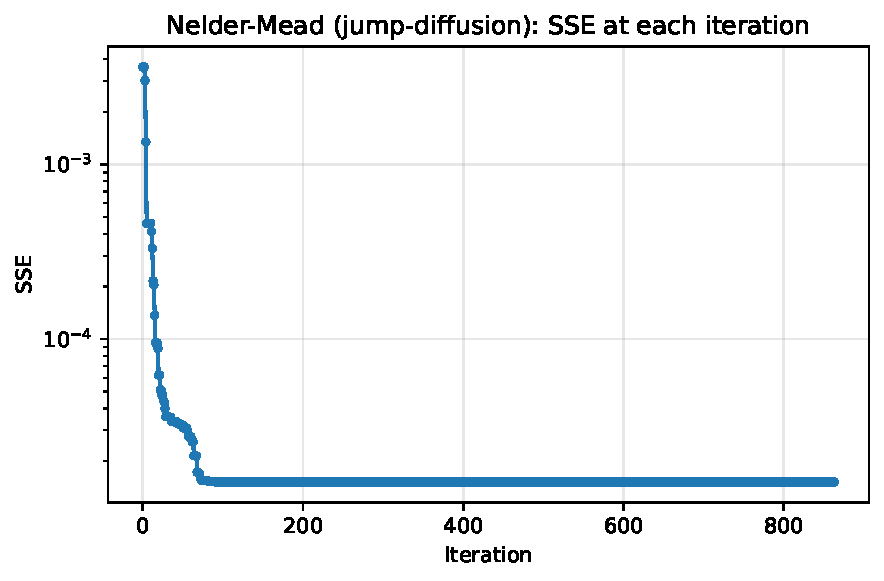
\includegraphics[width=0.65\textwidth]{figures/problem3_nelder_sse_jump}
  \caption{Nelder-Mead (jump-diffusion): SSE at each iteration.}
  \label{fig:problem3-nelder-jump}
\end{figure}

\begin{figure}[H]
  \centering
  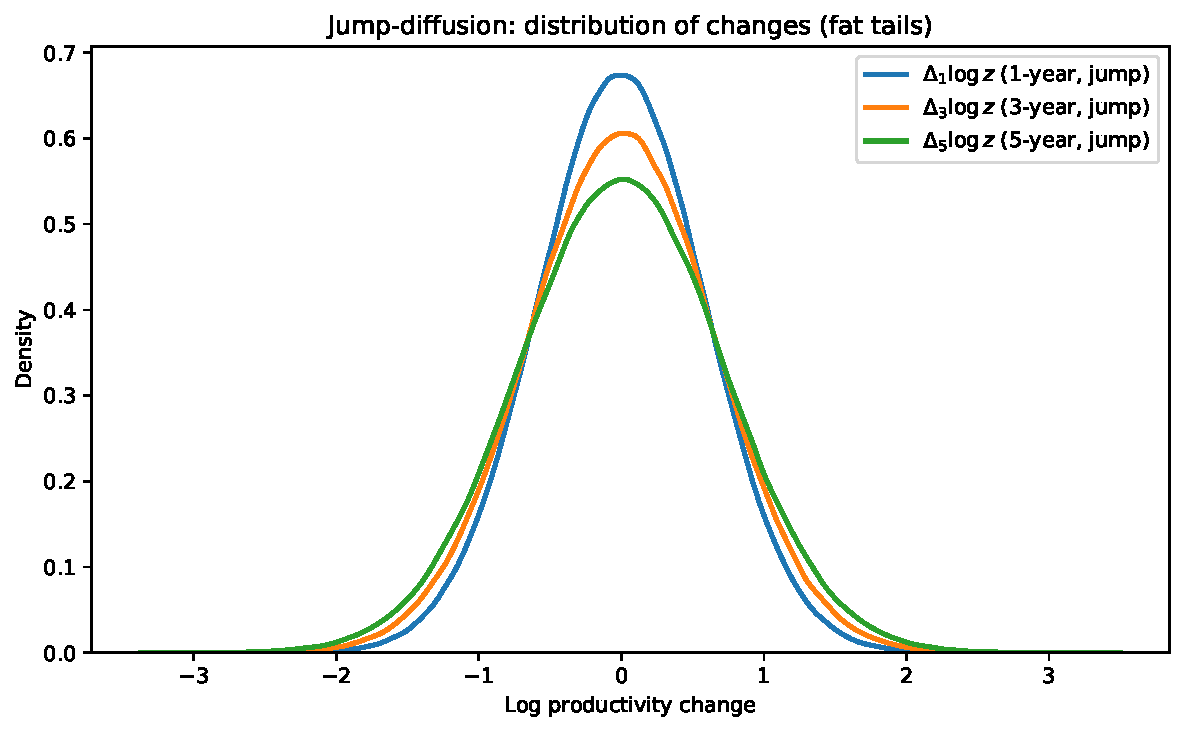
\includegraphics[width=0.75\textwidth]{figures/problem3_dlogz_jump}
  \caption{Jump-diffusion: distribution of log-productivity changes (fat tails).}
  \label{fig:problem3-dlogz-jump}
\end{figure}

\Cref{tab:problem3-moments} reports target vs.\ model moments for both specifications; \Cref{tab:problem3-parameters} reports the calibrated parameters. Tables are generated by \texttt{gen\_problem3\_figures.py}.

\begin{table}[H]
\centering
\caption{Target vs.\ model moments}
\label{tab:problem3-moments}
\begin{tabular}{lccc}
\toprule
Moment & Target & Baseline (AR(1)+noise) & Jump-diffusion \\
\midrule
$\operatorname{sd}(\log y)$ & 1.310 & 1.310 & 1.310 \\
$\operatorname{sd}(\Delta \log y)$ & 0.590 & 0.590 & 0.590 \\
$\Corr(y_t, y_{t-1})$ & 0.900 & 0.899 & 0.899 \\
$\Corr(y_t, y_{t-3})$ & 0.870 & 0.873 & 0.873 \\
$\Corr(y_t, y_{t-5})$ & 0.850 & 0.849 & 0.848 \\
\bottomrule
\end{tabular}
\end{table}

\begin{table}[H]
\centering
\caption{Calibrated parameters}
\label{tab:problem3-parameters}
\begin{tabular}{llc}
\toprule
Parameter & Model & Estimate \\
\midrule
$\rho$ & Baseline & 0.986 \\
$\sigma_u$ & Baseline & 0.210 \\
$\sigma_\varepsilon$ & Baseline & 0.390 \\
\midrule
$\rho$ & Jump-diffusion & 0.986 \\
$\sigma_\eta$ & Jump-diffusion & 0.198 \\
$\sigma_\varepsilon$ & Jump-diffusion & 0.390 \\
$\pi$ & Jump-diffusion & 0.050 \\
$\mu_J$ & Jump-diffusion & 0.000 \\
$\sigma_J$ & Jump-diffusion & 0.314 \\
\bottomrule
\end{tabular}
\end{table}

